\documentclass{school-22.211-notes}
\date{February 29, 2012}

\begin{document}
\maketitle



%%%%%%%%%%%%%%%%%%%%%%%%% Resonance Models Day 4 %%%%%%%%%%%%%%%%%%%%%%%%%%%%
\clearpage
\topic{Analytical Flux Models: Narrow Resonance vs. Wide Resonance}
%%%% 12 fall material %%%%
Reference: Alain Hebert's Applied Reactor Physics (p.199-202, Livolant-Jeanpierre approximation), Duderstadt's p.343-347. We only use these models for unresolved energy region nowadays. 

\begin{table}[ht]
  \centering
  \begin{tabular}{|c|p{2in}|p{2.5in}|} \hline
     & Narrow Resonance & Wide Resonance  \\ \hline
    Assumptions & $\Gamma_p \ll \overline{\Delta E}^R \Rightarrow \sigma_s^R = \sigma_{po}^R = $const. $\phi(u)=$ const.  & $ \overline{\Delta E}^R \ll \Gamma_p \ll \overline{\Delta E}^M \Rightarrow$ reaction rates $\sigma_s^R(u) \phi(u)$ = const. \\ \hline
    Fine structure $\phi(u)$ & $\displaystyle \frac{\sigma_{po}^R + \sigma_d}{\sigma_{t}^R (u) + \sigma_d} \approx \frac{\sigma_{po}^R + \sigma_d}{\sigma_{a}^R(u) + \sigma_{po}^R + \sigma_d }$ &  $\displaystyle \frac{\sigma_d}{\sigma_{t}^R (u) - \sigma_{s}^R (u) + \sigma_d} = \frac{\sigma_d}{\sigma_{a}^R (u) +  \sigma_d }$   \\ \hline
    Total $\Phi (E)$ &  $\displaystyle\frac{\Sigma_s^M + \Sigma_p^R}{\Sigma_t(E) E}$  & $\displaystyle\frac{\Sigma_s^M}{(\Sigma_t(E) - \Sigma_s^M(E))E}$ \\ \hline 
    Comments & Good for high energy.   & Ignore $\sigma_{po}^R$ b/c width.  \\ \hline
  \end{tabular}
  \caption{Comparison of Narrow and Wide Resonances}
\end{table}
As energy increases, $\overline{\Delta E}^R \up$, thus we use NR model for the unresolved resonance energy range. 

To start, recall the assumptions we made for slowing down equation in Section~\ref{slowing-down-from-te}: 
\begin{itemize}
\item Steady state.
\item Infinite medium: there is no spacial dependency. 
\item No external source. 
\item S-wave elastic scattering (that is isotropic in COM frame) for light nuclides, 
    \eqn{ \Sigma_s (E' \to E) &= \frac{\Sigma_s(E')}{(1-\alpha)E'} &\mbox{for } E < E' < \frac{E}{\alpha} }
\end{itemize}

For resonance models, we further consider, 
\begin{itemize}
\item Neutron flux has achieved its asymptotic behavior $\phi(E) \sim 1/E$ before reaching the resonance energy. 
\item The moderator has a constant $\sigma_s$ and a negligible $\sigma_a$ (at least over the resonance range): 
  \eqn{ \Sigma_t^M (E) \sim \Sigma_s^M (E) = \Sigma_{po}^M }
\end{itemize}

Recall the slowing down equation for the resonance region of $[1\eV, 0.1 \MeV]$ is, 
\eqn{ \Sigma_t (u) \Phi(u) &= \int_{u-\epsilon}^u \frac{1}{1 - \alpha} e^{-(u-u')} \Sigma_s (u') \Phi(u') \du' \label{resonance-sl-d-eqn} } 





\subtopic{Livolant-Jeanpierre Approximation}
This is the approach Prof. Forget followed in his lecture on 10/04/12. We manipulate Eq.~\ref{resonance-sl-d-eqn}:
\begin{itemize}
\item We facterize $\Phi(u) = \phi(u) \Psi(u)$, where $\phi(u)$ is the fine structure/self-shielding factor that models the resonances, $\Psi(u)$ is the flux outside the resonance (Hebert calls it `macroscopic flux', and it represents the asymptotic behavior of flux between resonances). 

\item For the resonant material (R) and the moderating material (M), we define the slowing down operator using the zeroth Legendre moment of the differential scattering cross section, 
\eqn{ R^R = \int_0^{\infty} \du' \Sigma_{s0}^R(u'\to u) \phi(\mu') }
\eqn{ R^M = \int_0^{\infty} \du' \Sigma_{s0}^M(u'\to u) \phi(\mu') }

\item Then the slowing down equation becomes, 
  \eqn{ (\Sigma_{t}^R (u) + \Sigma_{t}^M (u)) \Phi(u) &= \int_{u - \epsilon^R}^u \frac{ e^{-(u-u')} \Sigma_{s}^R (u') \Phi(u')}{1 - \alpha^R} \du' + \int_{u-\epsilon^M}^u \frac{e^{-(u-u')} \Sigma_{s}^M (u') \Phi(u')}{1 - \alpha^M}  \du'  }
  We do not know what $R^R$ is yet besides its definition,
  \eqn{  R^R \Phi(u) &= R^R \phi(u) \Psi(u) = \int_{u-\epsilon^R}^u \frac{1}{1-\alpha^R} e^{-(u-u')} \Sigma_{s}^R(u') \phi(u') \Psi(u') \du'  }
  But for $R^M$, we apply the $1/E$ flux between resonances and get rid of the $\phi(u)$ term, 
  \eqn{ R^M \Phi(u) &= \Sigma_{t}^M \Psi(u)  }

\item Then we can write (omitting $u$ dependency for simplicity) and cancel out $\Psi$ on both sides, 
  \begin{align}
    (\Sigma_{t}^M + \Sigma_t^R) \Psi \phi &= R^R \Psi \phi +  \Sigma_{t}^M \Psi  \\
   (\Sigma_t^M  + \Sigma_{t}^R ) \phi &=  R^R \phi + \Sigma_t^M  
  \end{align}

\item If we divide by $N^R$ (the resonance nuclide number density), we get 
  \eqn{ (\sigma_d + \sigma_{t}^R) \phi &= r^R \phi + \sigma_d }
\end{itemize}


There are a couple of ways to approximate $r^R \phi(u)$. 
\begin{enumerate}
\item Wide resonance assumes that the resonances are so large that we can assume the reaction rate (for the fine structure) is constant. 
\eqn{ r^R \phi(u) &= \int_{u-\epsilon^R}^u \frac{1}{1-\alpha^R} e^{-(u-u')} \overbrace{ \sigma_{s}^R (u') \phi(u')}^{\mathrm{constant}} \du' = \sigma_{s}^R (u) \phi(u)  }
Then we arrive at, 
\eqn{ \phi_{WR} (u) &= \frac{\sigma_d}{\sigma_{t}^R (u) - \sigma_{s}^R (u) + \sigma_d} = \frac{\sigma_d}{\sigma_{a}^R (u) +  \sigma_d } \label{WR-eqn} }
\begin{align}
\RIeff^{\gamma} &= \int \sigma_{\gamma}^R (u) \phi_{WR} (u) \du \\
&= \int \sigma_{\gamma}^R (u) \frac{\sigma_d}{\sigma_a^R(u) + \sigma_d} \du \\
&= \Ln{\frac{E_2}{E_1}} \frac{ \int \sigma_{\gamma}^R (E) \frac{\sigma_d}{\sigma_{a}^R(E) + \sigma_d} \frac{1}{E} \dE}{ \int \frac{\sigma_d}{\sigma_{a}^R(E) + \sigma_d} \frac{1}{E} \dE}
\end{align}
Comments:
\begin{itemize}
\item WR's $\sigma_s^R (u)$ term on the bottom is the resonant material's scattering cross section including both the potential scattering (hard sphere collision) and the compound nuclide scattering. That is, NR only accounts for the potential scattering cross section, whereas WR uses the entire scattering cross section. 

\item WR $\RI_{\eff}$ only depends on cross sections: $\sigma_d$ is assumed to be based on material composition of the reactor, and $\sigma_r(E)$ are from libraries. There is no need for flux spectrum. 

\item WR ignores U238 scattering, as there is no U238 scattering cross section in Eq.~\ref{WR-eqn}. Interpretation: the resonance width is large compare with the approximately 1\% energy lose upon a scattering, thus we can ignore the U238 scattering. To improve this approximation, sometimes people add the potential scattering of 11.39 barns. 

\item WR approximations match direct MC results near infinite dilution. 
\end{itemize}

\item Narrow resonance approximations assume resonance is very narrow, and a neutron is going to be out of the resonance upon one scattering, thus \textbf{cross section remains the same, thus $\Phi(E) \propto 1/E, \Phi(u) = $constant.} Thus we can write, 
\eqn{ r^R \phi(u) = \int_{u-\epsilon^R}^u \frac{1}{1- \alpha^R} e^{-(u-u')} \sigma_{s}^R (u') \Phi(u') \du' }
where $\Phi(u') = 1, \sigma_{s}^R (u')\approx \sigma_{po}^R$ potential scattering, also 
\eqn{ \int_{u-\epsilon}^u \frac{1}{1-\alpha^R} e^{-(u-u')} \du' = 1} 
Thus narrow resonance approximation leads to, 
\eqn{ r^R \phi(u) = \sigma_{po}^R}
That is, 
\eqn{ \sigma_{po}^R + \sigma_d &= (\sigma_d + \sigma_{t}^R (u)) \phi_{NR} (u) & \phi_{NR} (u) &= \frac{\sigma_{po}^R + \sigma_d}{\sigma_{t}^R (u) + \sigma_d} \approx \frac{\sigma_{po}^R + \sigma_d}{\sigma_{a}^R + \sigma_{po}^R + \sigma_d } }
\begin{align}
\RIeff^{\gamma} &= \int \sigma_{\gamma}^R (u) \phi_{NR} (u) \du \\
&= \int \sigma_{\gamma}^R (u) \frac{\sigma_{pot}^R + \sigma_d}{\sigma_a^R(u) + \sigma_{pot}^R + \sigma_d} \du \\
&= \Ln{\frac{E_2}{E_1}} \frac{ \int \sigma_{\gamma}^R (E) \frac{\sigma_{pot}^R + \sigma_d}{\sigma_{a}^R(E) + \sigma_{pot}^R + \sigma_d} \frac{1}{E} \dE}{ \int \frac{\sigma_{pot}^R + \sigma_d}{\sigma_{a}^R(E) + \sigma_{pot}^R + \sigma_d} \frac{1}{E} \dE}
\end{align}
Comments:
\begin{itemize}
\item NR approximation is good for higher energy. For instance, at 100 keV, scattering lose 1 keV, which is larger than the 25 eV spacing of \ce{^{238}U}. For fast reactor applications for instance narrow resonance is used a lot. 

\item However, the results on the slides come out to be that narrow resonance approximation is not really any better than the wide resonance approximation at higher energy, so there must be some other physics going on, see next section. 
\end{itemize}
\end{enumerate}


\clearpage
\subtopic{Duderstadt's Formalism} 
I find Duderstadt's (p.343-345) approach to NR \& WR as a helpful alternative without using the facterization of the flux. The rest of this section (including IR, comparison with MC, CASMO IR model) comes from Prof. Smith's 22.212 Lecture 7 on 02/27/2013. 
\begin{enumerate}
\item NR: assume the resonance width is small compared to the average energy loss in a collision with the resonant material (since the average energy loss $\sim \frac{(1-\alpha^R)E_0}{2}$, one can expect that NR is valid for high energy): 
  \eqn{ \Gamma_p \ll \overline{\Delta E}^R = \frac{1 - \alpha^R}{2} E_0  }
  Then the resonant scattering integral can be approximated by replacing $\Phi(E)$ by its asymptotic form: 
  \eqn{ \int_E^{E/\alpha^R} \dE' \frac{\Sigma_a^R(E') \Phi(E')}{(1 - \alpha^R) E'} \approx \frac{\Sigma_p^R}{1 - \alpha^R} \int_E^{E/\alpha^R} \frac{\dE'}{E'} \frac{1}{E'} = \frac{\Sigma_p^R}{E}  }
  Then the slowing down equation is, 
  \eqn{ \Sigma_t(E) \Phi(E) &= \frac{\Sigma_s^M + \Sigma_p^R}{E} & \Phi_{NR} (E) &= \frac{\Sigma_s^M + \Sigma_p^R}{\Sigma_t(E) E} }

\item WR: assume the resonance width is wide compared to the energy loss: 
  \eqn{ \overline{\Delta E}^R = \frac{1 - \alpha^R}{2} E_0 \ll \Gamma_p \ll  \overline{\Delta E}^M }
  WR can be referred to as `NR infinite mass absorber' (NRIM): resonant material is infinitely massive such that neutrons suffer no energy loss in a collision with the resonant materials. That is, as $A^R \to \infty, \alpha^R = (A^R - 1/A^R + 1)^2 \to 1$, and 
  \eqn{ \lim_{\alpha^R \to 1} \int_E^{E/\alpha^R} \frac{\Sigma_s^R (E') \Phi(E') \dE'}{(1-\alpha^R) E'} \to \Sigma_s^R (E) \Phi(E) \lim_{\alpha^R \to 1} \int_E^{E/\alpha^R} \frac{\dE'}{1 - \alpha^R} = \Sigma_s^R (E) \Phi(E) }
  Then slowing down equation becomes, 
  \eqn{ \Sigma_t(E) \Phi(E) &= \Sigma_s^R (E) \Phi(E) + \frac{\Sigma_s^M}{E} & \Phi_{WR} &= \frac{\Sigma_s^M}{(\Sigma_t(E) - \Sigma_s^M(E))E} }
  WR: intuitively, you cannot get in, and cannot get out, so the two sides cancel out. Once you get in, you pretty much just get absorbed. 

\item IR/Goldstein-Cohen Model: since isotopes are going to be somewhere between the two extremes, we consider a linear combination of $\psi_{NR}, \psi_{WR}$, 
\eqn{ \phi_{GC} (u) = \frac{\lambda_g \sigma_{po} + \sigma_d}{\sigma_{to}(u) - (1-\lambda_g) \sigma_{so}(u) + \sigma_d } }
where $\lambda_g$ depends on isotope and energy band. When $\lambda_g = 1$ we get the $\psi_{NR}$, $\lambda_g = 0$ we get the $\psi_{WR}$. Alternatively, we can discretize our energy group very finely, then we would not need any resonance models.

\item CASMO Intermediate Resonance Model: assume fixed temperature (900 K) and something else. FIXME. 
\end{enumerate}
\textbf{Compare with MC}\label{narrow-wide-compr}: As in Figure~\ref{wide-vs-narrow}, WR agrees pretty well with MC results without U238 potential scattering; NR agrees alright with the MC results with U238 potential scattering. Notice adding in scattering would change the low dilution factor results.

Compare with MC results using real U238 and U235 xs data, the real results fall between the wide and the narrow approximations for the high dilution factor; but for the low dilution factor, that is, when there are lots of resonance material (uranium), the physics gets complicated: 
\begin{itemize}
\item Non 1/E slowing down sources;
\item Non constant moderator xs;
\item Resonance scattering alters sources;
\item We may have multiple resonance in each RI group; that is, each of our RI does not include a single resonance anymore;
\item Resonance interference between \ce{^{235}U} and \ce{^{238}U}; eg: \ce{^{238}U}'s resonance spacing is 25 eV, whereas \ce{^{235}U}'s resonance spacing is 5 eV, that is, for each \ce{^{238}U} resonance, there are multiple \ce{^{235}U} resonances on top of it. 
\end{itemize}
\begin{figure}
  \centering
  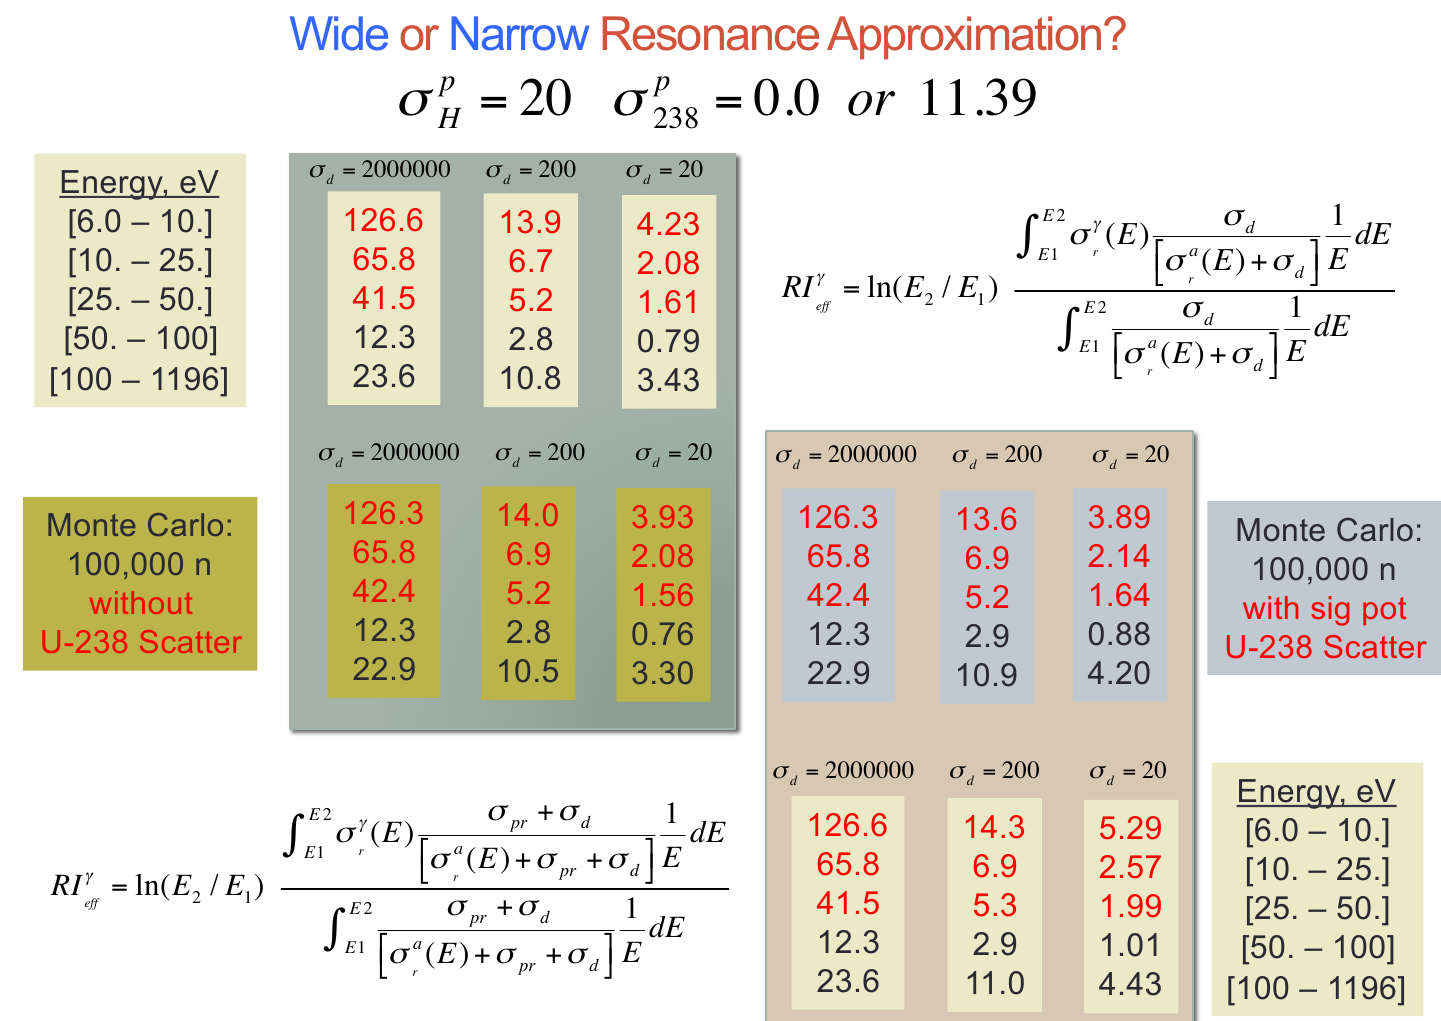
\includegraphics[width=5in]{images/r-m/narrow-vs-wide-resonance.png}
  \caption{Comparison Of Wide and Narrow Resonance Approximation} \label{wide-vs-narrow}
\end{figure}
\textbf{Helstrand Resonance Integral Measurements} (for isolated rod): LWR has a radius of 0.4 to 0.5cm, but a lattice of pins can be approximated with fatter isolated pins. So CASMO-5 results are about 2\% different from Helstrand RI measurements, which is equivalent to about 1\% difference in Doppler coefficients. 



\clearpage
\subtopic{Examples Using Resonance Models}
Prof. Forget described how to use resonance model in one group during lecture, and the two group problem showed up in a homework assignment. To start, recall that
\begin{itemize}
\item Flux facterization $\Phi(u) = \phi(u) \Psi(u)$ where $\phi$ is the fine structure function, $\Psi(u)$ is the flux outside the resonance. 
\item Dilution cross section: 
  \eqn{ \sigma_d = \frac{\Sum_{\mathrm{moderator}} N_m \sigma_m}{N_r} }
\item Narrow resonance approximation\footnote{the only energy/lethargy dependent term on the RHS should be $\sigma_{to}(u)$.}:
  \eqn{ \phi_{NR} (u) = \frac{\sigma_{po} + \sigma_d}{\sigma_d + \sigma_{to}(u)} }
\end{itemize}

There are two possibilites in using NR approximation to calculate the condensed cross section depends on the number of resonant isotopes: 
\begin{enumerate}
\item One resonant isotope. Assume we have \ce{H_2 O} and \ce{^{235} U}. 
\begin{align}
\sigma_d &= \frac{N_H \sigma_H + N_O \sigma_O}{N_U} 
\end{align}
We evaluate $\phi$ using narrow resonance approximation: 
  \eqn{ \phi_{NR} (u) = \frac{\sigma_{po} + \sigma_d}{\sigma_d + \sigma_{to}(u)} }
Then the flux-weighted resonant material cross section is,
\eqn{ \sigma_{U,g} = \frac{\int \sigma_{U}(u) \psi(u) \du}{\int \psi(u) \du} }

\item Multiple resonant isotopes. Assume we have \ce{H_2 O}, \ce{^{235}U}, and \ce{^{238} U}. 

  \textbf{Solution 1 (Livolant-Jeanpierre):} The idea is, we have to approximate $\sigma_d$ now that there are two resonant isotopes. The reason we emphasize on $\sigma_d$ is because in production tool we resolve the spectrum/group cross section for a number of dilution cross sections, and the data provided to the downstream applications would be a function of the diluion cross sections.  
  \begin{enumerate}
  \item Assume \ce{^{235} U} is the only resonant isotope, then we solve an energy independent $\sigma_d$ by 
    \eqn{ \sigma_d = \frac{N_{238} \bar{\sigma}_{238} + N_H \sigma_H + N_O \sigma_O}{N_{235} } }
    Then we solve for $\psi(u)$:
      \eqn{ \phi_{NR} (u) = \frac{\sigma_{po,235} + \sigma_d}{\sigma_d + \sigma_{to,235}(u)} \label{NR-flux-eqn}  }
    Then calculate the collapsed $\bar{\sigma}_{235}$:
    \eqn{ \bar{\sigma}_{235} = \frac{\int \sigma_{235} (u) \phi(u) \du}{\int \phi(u) \du}  \label{flux-collapse-235}  }
  \item Assume \ce{^{238} U} is the only resonant isotope. 
    \eqn{ \sigma_d = \frac{N_{235} \bar{\sigma}_{235} + N_H \sigma_H + N_O \sigma_O}{N_{238} } }
    Then we solve for $\psi(u)$:
      \eqn{ \phi_{NR} (u) = \frac{\sigma_{po,238} + \sigma_d}{\sigma_d + \sigma_{to,238}(u)} }
    Then calculate the collapsed $\bar{\sigma}_{238}$:
    \eqn{ \bar{\sigma}_{238} = \frac{\int \sigma_{238} (u) \phi(u) \du}{\int \phi(u) \du}   }
  \end{enumerate}
  Then we feed $\bar{\sigma}_{238}$ back into step 1 and repeat the process until $\bar{\sigma}_{235}, \bar{\sigma}_{238}$ converge, which happen fairly fast with a simple resonance. 


\textbf{Solution 2 (Dederstadt)}: \\
In Eq.~\ref{flux-collapse-235}, $\phi(u)$ shows up in both the top and the bottom of the equation, so if we scale $\phi(u)$ by any non-energy dependent term as they would just cancel out, the solution would not change. Recall $\phi(u)$ as in Eq.~\ref{NR-flux-eqn}, the top $\sigma_{po,r} + \sigma_d$ is energy-independent, and $N_r$ is energy-independent as well, that is, 
\eqn{ \phi_{NR} (u) = \frac{\sigma_{po,r} + \sigma_d}{\sigma_d + \sigma_{to,r}(u)} \to \frac{1}{\sigma_d + \sigma_{to,r}(u)} \to  \frac{1}{N_r \sigma_d + N_r \sigma_{to,r}(u)} \to \frac{1}{\Sum_{\mathrm{moderators}} N_m \sigma_m + N_r \sigma_{to,r}(u)} }
Then the total flux is fine structure times a $1/E$ dependency, 
\eqn{ \Phi (E) = \frac{1}{E \left[ \Sum_{\mathrm{moderators}} N_m \sigma_m + N_r \sigma_{to,r}(E)\right]} }
Then we don't have to compute $\sigma_d$ anymore. For each resonant isotope, the three steps becomes two steps: calculating $\Phi$ using last step's condensed cross section, and update this step's condensed cross section with $\Phi$-collapsed cross section. 

So effectively narrow resonance suggest, 
\eqn{ \Phi (E)  = \frac{1}{E \Sigma_t (E)} }
\end{enumerate}


\clearpage
\topic{Procedure for Generating Multigroup Cross Sections}
How does a production tool uses resonance parameters?\\
\textbf{Normal procedure} for generating multi-group xs in a code like NJOY includes:
\begin{enumerate}
\item Use code to Doppler broaden cross sections for each resonance isotope for range of temperatures (eg, 300, 600, 900, 2000K); 
\item Use code to apply the narrow or wide resonance models for a range of dilution xs (eg, 20000, 2000, 200, 20 barns); 
\item Edit RIs or multi-group xs for your desired energy structure; 
\item Build tables of xs vs. dilution xs and temperature;
\item For downstream computations, interpolate for the dilution cross section and temperature of each material in the simulation to obtain accurate multigroup cross sections for that specific applications. 
\end{enumerate}
Problem with this approach: cannot take into account resonance interference from multiple isotopes' resonances in the same RI group. There are other assumptions

\textbf{A better procedure} for generating multi-group cross sections includes:
\begin{enumerate}
\item Same;
\item Use code to solve real neutron slowing down problem for a range of dilution cross sections (eg, 20000, 2000, 200, 20 barns);
\item Consider including a mix of resonance absorbers to make the spectrum as appropriate to the desired application as possible. For instance we put in U238 as admixed to take into account the first order effect of the interference between U238 and other resonance materials. 
\item Same;
\item Same;
\item Same.
\end{enumerate}
Still we have to be careful about the assumptions we made (constant amount of U238, so would not work well with reactors with no U238). 

For downstream applications that require cross section data, for each resonance group,
\begin{enumerate}
\item For each composition, evaluate the material temperature and isotopic densities. 
\item Evaluate Dancoff from pin diameter, lattice pitch, etc. 
\item Compute the escape cross section for each resonance absorber.
\item Evaluate group cross section (or RI) using Dancoff, potential and escape cross sections by interpolating cross section (or RI) tables at appropriate temperatures. 
\end{enumerate}
For real application, it is rarely possible to just use someone else's cross section table; we almost certainly need to generate xs suitable for our application. 








\end{document}
